\section{Package View}
\begin{figure}[h!]
\begin{center}
	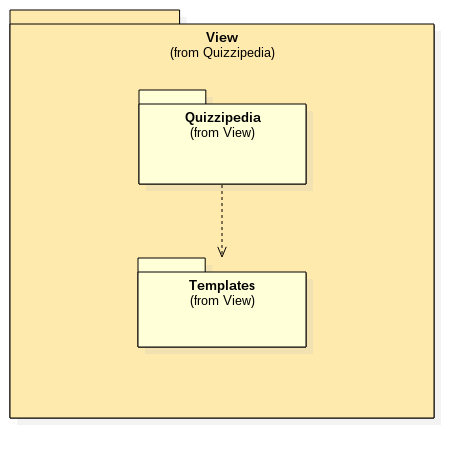
\includegraphics[scale=0.7]{../images/ViewPackage.png}
\end{center}
\end{figure}

\subsection{View::Quizzipedia}
\begin{itemize}
\item\textbf{Funzione del componente:} wrapper degli elementi comuni a tutte le pagine
\item\textbf{Relazioni d'uso con altre componenti:} 
\begin{itemize}
	\item View::Templates::quizHome
\item View::Templates::quizHome
\item View::Templates::quizList
\item View::Templates::quizResults
\item View::Templates::quizStatistics
\item View::Templates::quizzipedia
\item View::Templates::searchForm
\item View::Templates::topbar
\item View::Templates::userProfile
\item View::Templates::navbar
\item View::Templates::question
\item View::Templates::questionForm
\item View::Templates::questionList
\item View::Templates::quiz
\item View::Templates::quizCompilation
\item View::Templates::quizCreationForm
\item ViewModel::Router::Router
\end{itemize}
\end{itemize}
\newpage

\subsection{View::Templates}
\subsubsection{View::Templates::quizHome}
\begin{itemize}
\item\textbf{Funzione del componente:} genera la pagina di benvenuto\\
\item\textbf{Relazioni d'uso con altre componenti:} ViewModel::Controller::QuizHome\\
\end{itemize}
\subsubsection{View::Templates::quizList}
\begin{itemize}
\item\textbf{Funzione del componente:} permette visualizzazione e interazione di una lista di questionari\\
\item\textbf{Relazioni d'uso con altre componenti:} ViewModel::Controller::QuizList\\
\end{itemize}
\subsubsection{View::Templates::quizResults}
\begin{itemize}
\item\textbf{Funzione del componente:} visualizza i risultati ottenuti in seguito alla compilazione di un quiz\\
\item\textbf{Relazioni d'uso con altre componenti:} ViewModel::Controller::QuizResults\\
\end{itemize}
\subsubsection{View::Templates::quizStatistics}
\begin{itemize}
\item\textbf{Funzione del componente:} permette la visualizzazione delle statistiche generali di una domanda\\
\item\textbf{Relazioni d'uso con altre componenti:} ViewModel::Controller::QuizStatistics\\
\end{itemize}
\subsubsection{View::Templates::searchForm}
\begin{itemize}
\item\textbf{Funzione del componente:} visualizza una form per l’inserimento dei dati desiderati e l’avvio della ricerca\\
\item\textbf{Relazioni d'uso con altre componenti:} ViewModel::Controller::SearchForm\\
\end{itemize}
\subsubsection{View::Templates::topbar}
\begin{itemize}
\item\textbf{Funzione del componente:} Fornisce il menù orrizontale con cui l'utente può interfacciarsi con il sistema\\
\item\textbf{Relazioni d'uso con altre componenti:} ViewModel::Controller::TopBar\\
\end{itemize}
\subsubsection{View::Templates::userProfile}
\begin{itemize}
\item\textbf{Funzione del componente:} permette la visualizzazione e l'interazione dell'utente con il proprio profilo e le funzionalità da esso offerto\\
\item\textbf{Relazioni d'uso con altre componenti:} ViewModel::Controller::UserProfile\\
\end{itemize}
\subsubsection{View::Templates::navbar}
\begin{itemize}
\item\textbf{Funzione del componente:} Fornisce un menù laterale che facilita l'interazione dell'utente con l'applicazione\\
\item\textbf{Relazioni d'uso con altre componenti:} ViewModel::Controller::NavBar\\
\end{itemize}
\subsubsection{View::Templates::question}
\begin{itemize}
\item\textbf{Funzione del componente:} permette la visualizzazione di una singola domanda\\
\item\textbf{Relazioni d'uso con altre componenti:} ViewModel::Controller::Question\\
\end{itemize}
\subsubsection{View::Templates::questionForm}
\begin{itemize}
\item\textbf{Funzione del componente:} visualizza il form utilizzabile sia per la creazione che per la modifica di una domanda\\
\item\textbf{Relazioni d'uso con altre componenti:} ViewModel::Controller::QuestionForm\\
\end{itemize}
\subsubsection{View::Templates::questionList}
\begin{itemize}
\item\textbf{Funzione del componente:} visualizza una lista di domande\\
\item\textbf{Relazioni d'uso con altre componenti:} ViewModel::Controller::QuestionList\\
\end{itemize}
\subsubsection{View::Templates::quiz}
\begin{itemize}
\item\textbf{Funzione del componente:} visualizza un quiz inserito in una lista\\
\item\textbf{Relazioni d'uso con altre componenti:} ViewModel::Controller::Quiz\\
\end{itemize}
\subsubsection{View::Templates::quizCompilation}
\begin{itemize}
\item\textbf{Funzione del componente:} \\
\item\textbf{Relazioni d'uso con altre componenti:} ViewModel::Controller::QuizCompilation\\
\end{itemize}
\subsubsection{View::Templates::quizCreationForm}
\begin{itemize}
\item\textbf{Funzione del componente:} visualizza il form di creazione di un questionario\\
\item\textbf{Relazioni d'uso con altre componenti:} ViewModel::Controller:QuizCreationForm:\\
\end{itemize}




